\documentclass[a4paper,12pt]{article}
\usepackage{float}
\usepackage{gensymb}
\usepackage[left=2cm,right=2cm,top=2cm,bottom=2cm]{geometry}
\usepackage{cmap}					% поиск в PDF
\usepackage[T2A]{fontenc}			% кодировка
\usepackage[utf8]{inputenc}			% кодировка исходного текста
\usepackage[english,russian]{babel}	% локализация и переносы
\usepackage{amsmath,amsfonts,amssymb,amsthm,mathtools}
\usepackage[warn]{mathtext}
\usepackage{graphicx}
\usepackage{xcolor}
\usepackage{adjustbox}
\usepackage{soul}
\usepackage{listings}
\graphicspath{{C:\Users\123\Desktop}}
\begin{titlepage}
	\centering
	\vspace{5cm}
	{\scshape\LARGE Московский физико-технический институт \par}
	\vspace{4cm}
	{\scshape\Large Черновик диплома \par}
	\vspace{1cm}
        
           	{\huge\bfseries  Численное моделирование воздействия вибрационной нагрузки на образец в трёхмерном случае. \par} 
        

	\vspace{1cm}
	\vfill
\begin{flushright}
	{\Large }\par
	\vspace{0.3cm}
	{\large  \par
                 
 } \par

\end{flushright}
	

	\vfill

% Bottom of the page
	Долгопрудный, 2021 г.
\end{titlepage}

\begin{document}
\section{Постановка задачи}
Есть пластина, она занимает объем $\overline{\Omega} \times [-\frac{1}{2}h, \frac{1}{2}h] \subset \mathbb{R}^3$, h - толщина пластины. $\Omega$ - срединная плоскость Граница пластины состоит из двух частей:
\begin{equation}
    \partial \Omega = \text{Г}_{\text{с}} \cup \text{Г}_{\text{f}}
\end{equation}
где $\text{Г}_{\text{с}}$ - закрепленный конец, $\text{Г}_f$ - свободный конец
\begin{figure}[H]
	\begin{center}
		\includegraphics[width = 0.7\textwidth]{tp3d.png}
		\caption{Модель пластины в 3D}
	\end{center}
\end{figure}

\begin{figure}[H]
	\begin{center}
		\includegraphics[width = 0.7\textwidth]{tp2d.png}
		\caption{Модель пластины в 2D}
	\end{center}
\end{figure}
\textcolor{red}{Пока техал заметил, что gmsh считает 2d поверхностью только 1 плоскость, ту, которой дана 2D physical group, надеюсь это норм}
\begin{figure}[H]
	\begin{center}
		\includegraphics[width = 0.9\textwidth]{tp3d.1.png}
		\caption{Модель пластины в 3D issue}
	\end{center}
\end{figure}

уравнение динамики для пластины:
\begin{equation}
2e\rho\ddot{\omega}^0 - \frac{2e^3}{3}\rho\Delta\ddot{\omega}^0 - div \: div \: \textbf{M} = f,
\end{equation}
где $ e = \frac{1}{2}h $,  $\rho$ - плотность материала, $f$ - внешняя нагрузка, $\textbf{M}$ - тензор моментов:
\begin{equation}
M =     
\begin{pmatrix}
M_{xx} & M_{xy}\\
M_{xy} & M_{yy} 
\end{pmatrix}
 = \int_{z = -\frac{h}{2}}^{z =\frac{h}{2}} z^2 \begin{pmatrix}
\sigma_{xx} & \sigma_{xy}\\
\sigma_{xy} & \sigma_{yy} 
\end{pmatrix}\,dz\
\end{equation}
Компоненты тензора моментов можно выразить, используя закон Гука:
\begin{equation}
    \begin{pmatrix}
        M_{xx} \\
        M_{yy} \\
        M_{zz} \\ 
    \end{pmatrix}
    = 
    \begin{pmatrix}
    D_{11} & D_{12} & D_{16} \\
    D_{12} & D_{22} & D_{26} \\
    D_{16} & D_{26} & D_{66} \\
    \end{pmatrix}\begin{pmatrix}
        \frac{\partial^2}{\partial x^2} \\
        \frac{\partial^2}{\partial y^2} \\
        \frac{\partial^2}{\partial z^2} \\ 
    \end{pmatrix} = \frac{2e^3}{3}
    \begin{pmatrix}
    C_{11} & C_{12} & C_{16} \\
    C_{12} & C_{22} & C_{26} \\
    C_{16} & C_{26} & C_{66} \\
\end{pmatrix}
    \begin{pmatrix}
        \frac{\partial^2}{\partial x^2} \\
        \frac{\partial^2}{\partial y^2} \\
        \frac{\partial^2}{\partial z^2} \\ 
    \end{pmatrix}
\end{equation}



Задачу можно сформулировать в следующем виде:

        
\begin{equation}
\rho\ddot{\omega}^0 - \frac{1}{3}\rho e^2\Delta\ddot{\omega}^0 - \frac{1}{2e}div \: div \: \mathcal{D}\nabla \nabla \omega^0 = \frac{1}{2e}f,
\end{equation}
\begin{equation}
\begin{cases}
    \omega^0 = g & \text{на $\text{Г}_c$}  \\
    \frac{\partial\omega^0}{\partial n} = 0 & \text{на $\text{Г}_c$} \\
\end{cases}
\end{equation}

\begin{equation}
\begin{cases}
    \frac{2}{3}e^3\rho \frac{\partial}{\partial n} \ddot{\omega}^0  + div  \: \textbf{M} \cdot \textbf{n} + \frac{\partial}{\partial \tau}(\textbf{Mn} \cdot\tau)& \text{на $\text{Г}_f$} \\
     \textbf{Mn}\cdot \tau= 0 & \text{на $\text{Г}_f$} \\
\end{cases}
\end{equation}

где $\mathcal{D}$ - тензор четвертого ранга:
\begin{equation}
\mathcal{D} = 
\begin{pmatrix}
    D_{11} & \frac{1}{2}D_{16} & 0 &  D_{16} & \frac{1}{2}D_{66} &0 &0 &0 & 0 \\
    \frac{1}{2}D_{16} & D_{12} & 0 & \frac{1}{2}D_{66} & D_{26} & 0 & 0&0 &0 \\
    0&0&0&0&0&0&0&0&0\\
    D_{16} & \frac{1}{2}D_{66} & 0 & D_{12} & \frac{1}{2}D_{26} & 0 &0 &0&0 \\
    \frac{1}{2}D_{66} & D_{26} & 0 & \frac{1}{2}D_{26} & D_{22} & 0 &0 &0&0 \\
    0&0 &0 &0 &0 &0 &0 &0 &0 \\
    0&0 &0 &0 &0 &0 &0 &0 &0 \\
    0&0 &0 &0 &0 &0 &0 &0 &0 \\
    0&0 &0 &0 &0 &0 &0 &0 &0 \\
    
\end{pmatrix}
\end{equation}
\textcolor{red}{ Для 2D - зачернуть все нули}

Пользуясь теоремой о дивергенции  $\int_{\Omega}(div \:\overline{p}) v) + \int_\Omega\overline{p}v = \int_{\partial\Omega} (\overline{p} \cdot \overline{n}) v $ 
% и формулой Грина $\int_\Omega (\Delta u )v  + \int_\Omega \nabla u \nabla v = \int_{\partial \Omega} (\partial_n u) v$ 
\begin{align}
\int_\Omega (\rho \omega^2 (u \nu + \frac{1}{3}e^2 \Delta u \nu) + \frac{1}{2e} div \: div \: \hat{\mathcal{D}} \nabla \nabla u \nu -f\nu)d\Omega = \\
=\int_\Omega (\rho \omega^2 (u \nu - \frac{1}{3}e^2 \nabla u \nabla \nu) + \frac{1}{2e} div \: div \: \hat{\mathcal{D}} \nabla \nabla u \nu -f\nu)d\Omega + \int_{\partial \Omega} \nabla u \cdot \overline{\textbf{n}}\nu = \\
=\int_\Omega (\rho \omega^2 (u \nu - \frac{1}{3}e^2 \nabla u \nabla \nu) - \frac{1}{2e}  div \: \hat{\mathcal{D}} \nabla \nabla u \nabla \nu -f\nu)d\Omega +\int_{\partial \Omega} \frac{1}{2e} \overline{\textbf{n}} \: div \:  \hat{\mathcal{D}} \nabla \nabla u  \nu  = \\
=\int_\Omega (\rho \omega^2 (u \nu - \frac{1}{3}e^2 \nabla u \nabla \nu) - \frac{1}{2e} \hat{\mathcal{D}} \nabla \nabla u : \nabla \nabla \nu -f\nu)d\Omega - \int_{\partial \Omega} \frac{1}{2e} \overline{\textbf{n}} \: \hat{\mathcal{D}} \nabla \nabla u \nabla \nu = \\
=\int_\Omega (\rho \omega^2 (u \nu - \frac{1}{3}e^2 \nabla u \nabla \nu) + \frac{1}{2e} \hat{\mathcal{D}} \nabla \nabla u : \nabla \nabla \nu -f\nu)d\Omega = 0  
\end{align}
Будем считать, что закрепленная граница колеблется с известной частотой и амлитудой
\begin{equation}
    g(x,y,z,t) = g_\omega(x,y,z)\cdot e^{i\omega t}
\end{equation}
Задача линейная, следовательно решение можно представить в виде
\begin{equation}
    \omega^0 = \omega^0_{part} +  \sum_{i=0}^{\infty} C_i \omega^0_i 
\end{equation}
Т.к присутствует потеря энергии, считаем, что вторым слагаемым по прошествии достаточно долгого времени можно пренебречь.
\par Частное решение будем искать в виде
\begin{equation}
    \omega_{part} = u(x,y,z,\omega) \cdot e^{i\omega t}
\end{equation}
Модель демпфирования заключается в представлении тензора \mathcal{D}:
\begin{equation}
    \mathcal{\hat{D}_\alpha} = \mathcal{D}(1 + i\beta_\alpha)
\end{equation}
где $\beta_\alpha$ - коэффициент потерь, $\alpha \in  \{11,12,16,22,26,66\}$.
Будем считать для численного расчета, что $ g \equiv 1$.
Слабая формулировка проблемы может быть сформулирована следующим образом: Найти $u \in H^2_2(\Omega)$ такое что $u|_{\text{Г}_c} = 1$, $\frac{\partial u}{\partial n }|_{\text{Г}_c} = 0$ и для всех $\nu \in H^2_2(\Omega)$ удовлетворяющих $\nu|_{\text{Г}_\text{c}}  = \frac{\partial \nu}{\partial n}|_{\text{Г}_\text{с}}= 0$ выполнено
\begin{equation}
\int_\Omega (\rho \omega^2 (u \nu + \frac{1}{3}e^2 \nabla u \nabla \nu) + \frac{1}{2e}\hat{\mathcal{D}} \nabla \nabla u : \nabla \nabla \nu -f\nu)d\Omega = 0    
\end{equation} 
Решение Аппроксимируется как линейная комбинация базисных функций $h_i$
\begin{equation}
    u = \sum_{i \in I}u_ih_i + \sum_{k \in D}g_kh_k
\end{equation}
I - подмножество индексов базисных функций, которые равны 0 на $\text{Г}_\text{с}$. D - множество индексов базисных функций, которые аппроксимируют граничное условие Дирихле. \textcolor{red}{ И тут я понял, что с граничными условиями что-то не так...}

\begin{lstlisting}

\end{lstlisting}

\section{ГУ. Попытка натянуть сову на глобус}
1. Граничное условике Дирихле на закрепленном конце (44-45):
\begin{lstlisting}
u_D = np.array([1], dtype=default_scalar_type)
bc = fem.dirichletbc(u_D, 
        fem.locate_dofs_topological(V, fdim, ft.find(1)), V)
\end{lstlisting}
2. Граничное условие Неймана на закрепленном конце (второе уравнение системы (6)): в коде не отражается т.к. условия Неймана в фениксе задаются интегралом в линейной форме (правой части) -> интеграл от 0 ни на что не влияет

\par
3. Равенство нулю тангенсального напряжения на свободном конце (система (7)):
\begin{equation}
    \textbf{M} \textbf{n} \cdot \tau = D \nabla \nabla u \cdot \textbf{n} \tau  = 0 
\end{equation}
Аналогично п.2
\par
\textcolor{red}{Выглядят, конечно, п.2 и п.3 неправдоподобно, но $\pm$ согласутеся с тем, что я вычитал на формумах. А вот как занулить $\nabla \nu$ на границе... Даже если это сработало в п.3 и п.2, то сейчас кажется что интеграл по границе в (12) точно не поможет, проблема в том, что других механизмов как задать условие Неймана я не нашел. }


\section{Тем не менее, что-то посчиталось}
В коде слабая формулировка задается следующим образом (106-110):
\begin{lstlisting}
#Bilinear form
a = 2*e*(-rho * omega ** 2 * ( (ufl.inner(u, v) ) \
+ 1 / 3 * e ** 2 * ufl.inner(grad(u)[0,:], grad(v)[0,:]) ) \
- 1/(2*e)*ufl.inner(D_2d,ufl.outer(grad(grad(u)[0,:]),
grad(grad(v)[0,:]))))*ufl.dx
# Linear form
L = ufl.inner(f,v[0])*ufl.dx
\end{lstlisting}

\begin{figure}[H]
	\begin{center}
		\includegraphics[width = 0.7\textwidth]{afc_P3_D2.find.png}
		\caption{АЧХ на P3 в 2D}
	\end{center}
\end{figure}

\begin{figure}[H]
	\begin{center}
		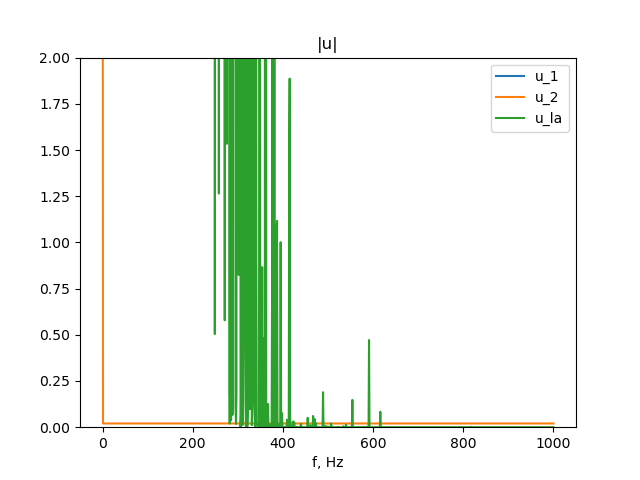
\includegraphics[width = 0.7\textwidth]{afc_P3_D3.png}
		\caption{АЧХ на P3 в 3D}
	\end{center}
\end{figure}

\begin{figure}[H]
	\begin{center}
		\includegraphics[width = 0.7\textwidth]{new_afc_P2.find.png}
		\caption{АЧХ на P2 в 2D}
	\end{center}
\end{figure}


\textcolor{red}{Продолжение следует... Я пока попытаюсь починить ГУ}


\end{document}